%======================================================================
\section{Track UIX --- UI and styling (after M2)}\label{sec:uix}
%======================================================================

Styling comes after the functional tracks, as decided. Three epics are already merged or under way: the
preference pack and viewport styling (\#8), the macOS title bar and overlay tree (\#6), and the timeline
spike (\#7). The rest of this chapter is the Fusion-style layout from the earlier UI plan, kept as the
\emph{starting brief} for the redesign. Its mocks are redrawn in \eref{UIX-09}; the first round is section~\ref{sec:ui-design}.

\begin{epic}{UIX-01}{Theme, pref pack \& viewport styling}{UI}{\stDone}{FCB-P1-01..05, P1V-01..07, P1V-10..18}
Merged (\#8). Follow-ups: the anti-aliasing check on Retina, and the mechanical user's try-out and sign-off.
\end{epic}
\begin{epic}{UIX-02}{macOS title bar}{UI}{\stDone}{FCB-P1F-01..05, P1F-26}
Merged (\#6): unified title bar and native window buttons behind a preference.
\end{epic}
\begin{epic}{UIX-03}{Browser (overlay model tree)}{UI}{\stProg}{FCB-P1F-06..14, P1F-27}
Prefs/QSS version merged (\#6). The free-floating panel (any inset, free height) needs a small
\code{OverlayManager} patch (FCB-P1F-11). Also fix it not showing on first run (\eref{FND-06}).
\end{epic}
\begin{epic}{UIX-04}{History timeline}{UI}{\stProg}{FCB-P1F-15..25, P1F-28}
Spike and mock merged (\#7). Remaining: the full bar with marker drag, edit, suppress and reorder (where
feasible), one-row layout, playback buttons, and a path into core.
\end{epic}
\begin{epic}{UIX-05}{Workspaces \& tabs (Fusion naming)}{UI}{\stTodo}{(new, from the UI plan)}
Design / Simulation / Manufacture / Drawing workspaces; Design tabs Solid, Surface, Mesh, Sheet Metal and
Utilities, plus a contextual Sketch tab. Extra workbenches are toggled in Preferences.
\end{epic}
\begin{epic}{UIX-06}{Toolbar \& panels}{UI}{\stTodo}{(new, from the UI plan)}
Captioned tool groups at one icon size, a floating command dialog, document tabs on top, and a one-row timeline.
\end{epic}
\begin{epic}{UIX-07}{Task panel polish}{UI}{\stTodo}{FCB-P1-06/07/08}
Sketcher, PartDesign and TechDraw dialogs.
\end{epic}
\begin{epic}{UIX-08}{Matcap shading}{UI}{\stTodo}{FCB-P1V-08/09/13/14/15}
A matcap draw style behind a preference; with the preference off, rendering is stock.
\end{epic}
\begin{epic}{UIX-09}{Fresh UI design \& re-render figures}{UI}{\stTodo}{(new)}
A new visual design for the whole application, then regenerate every figure in this document with the scripts
in \file{scripts/}.
\end{epic}

\subsection{Starting brief: review of the current window}

\begin{figure}[ht]
\centering
\begin{tikzpicture}
  \node[anchor=south west,inner sep=0] (img) at (0,0) {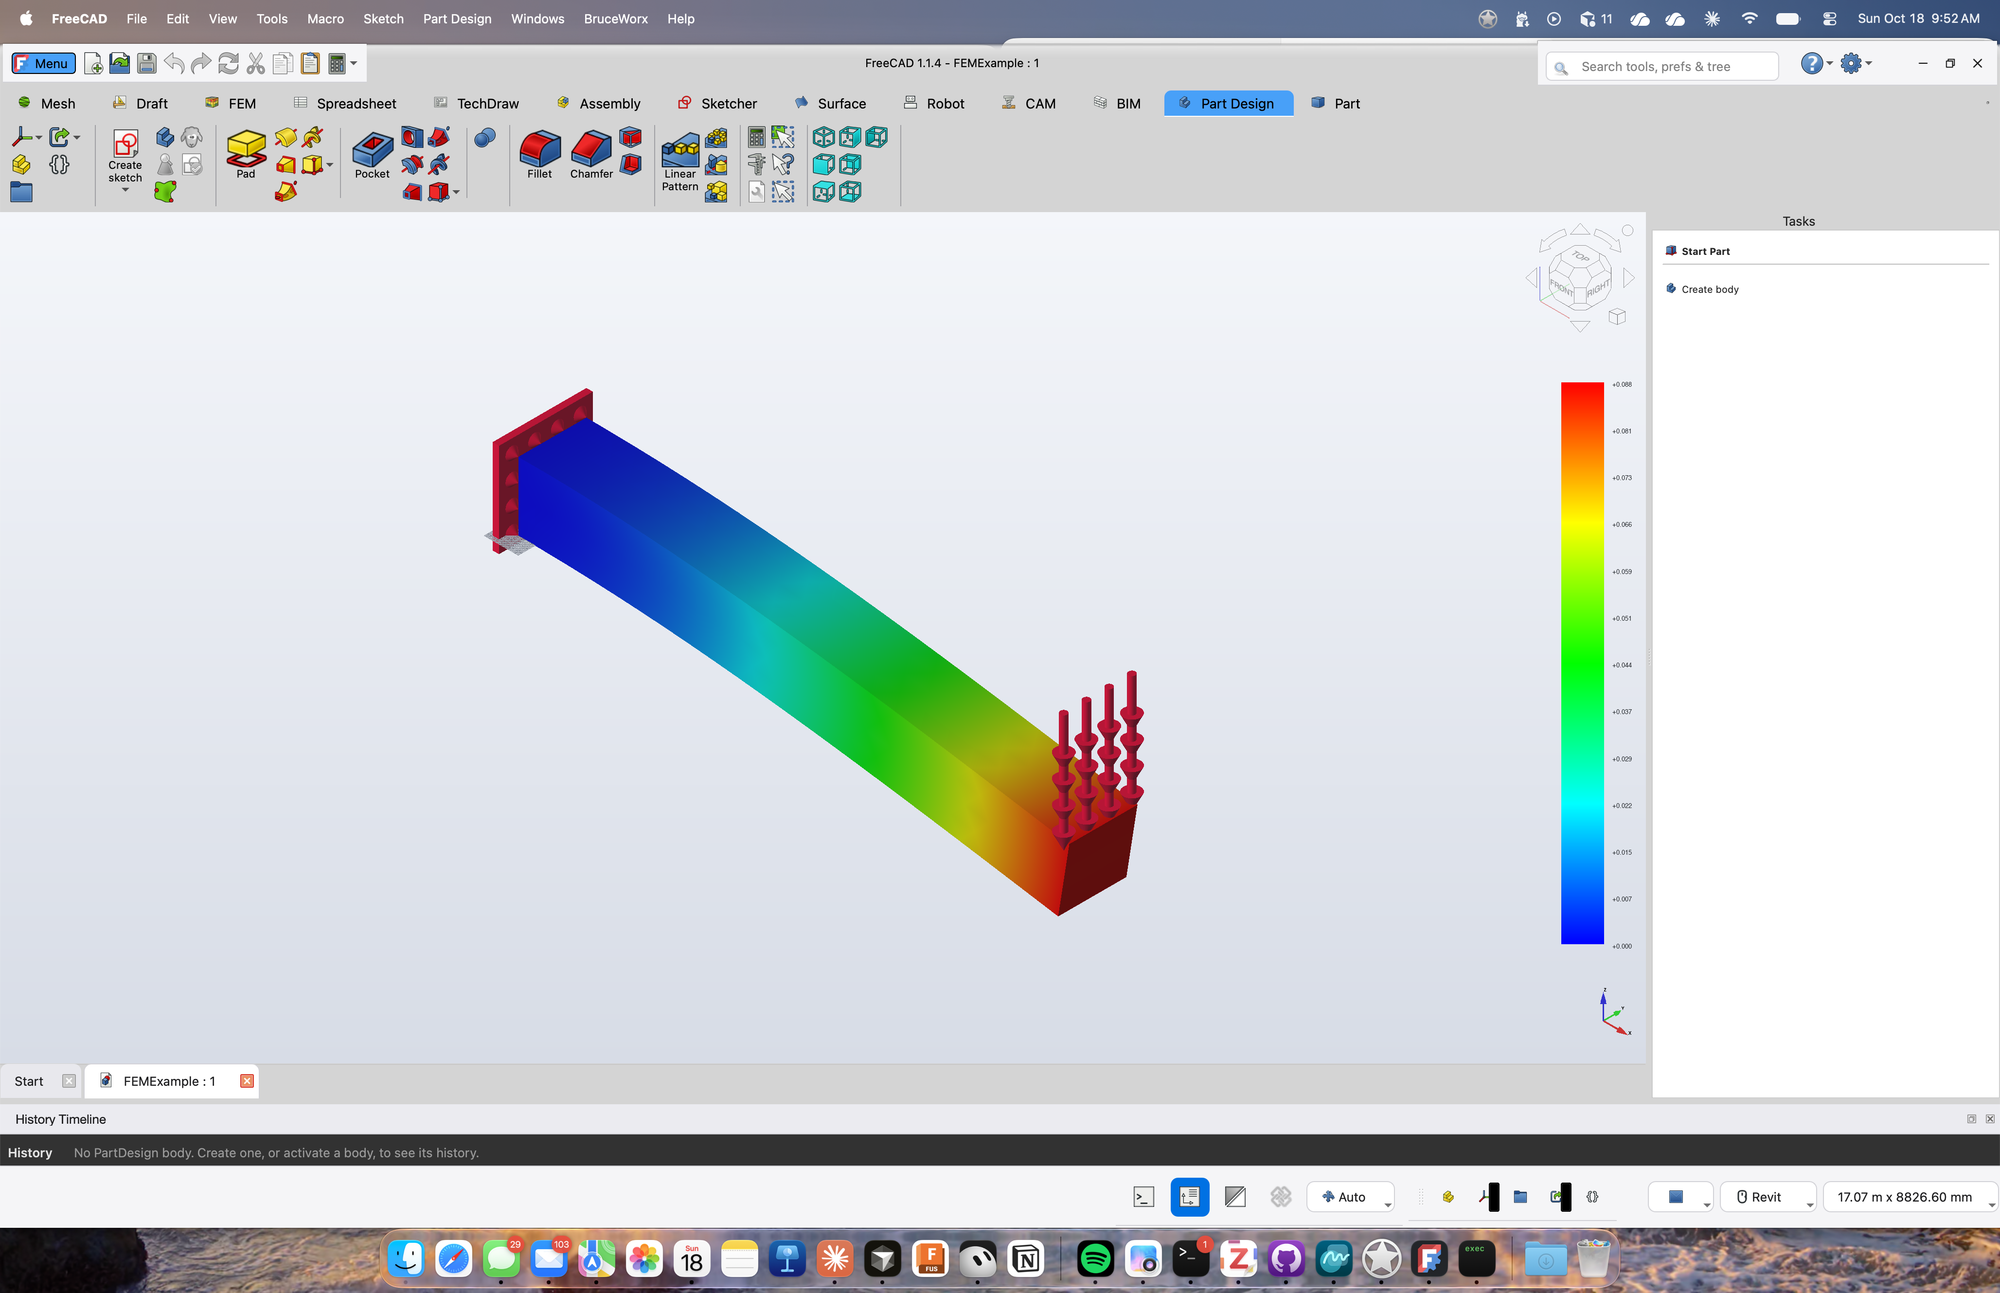
\includegraphics[width=\linewidth]{fig/before.png}};
  \begin{scope}[x={(img.south east)},y={(img.north west)}]
    \foreach \n/\x/\y in {1/0.36/0.92, 2/0.23/0.87, 3/0.90/0.77, 4/0.07/0.73, 5/0.17/0.165, 6/0.29/0.11, 7/0.53/0.075}
      \node[circle,fill=bwred,text=white,font=\scriptsize\bfseries,inner sep=1.2pt,minimum size=13pt,draw=white,line width=0.8pt] at (\x,\y) {\n};
  \end{scope}
\end{tikzpicture}
\caption{The window as of 18 Oct 2026, with issues numbered.}
\label{fig:before}
\end{figure}

\begin{center}
\small
\begin{tabularx}{\linewidth}{@{}cXX@{}}
\toprule
\# & Issue & Cause / fix\\
\midrule
\marker{1} & 13 workbench tabs & Pack trim not applied (\eref{FND-06}); replaced by workspaces (\eref{UIX-05})\\
\marker{2} & Icon grid in mixed sizes, few labels & Captioned groups, one size (\eref{UIX-06})\\
\marker{3} & Full-height Tasks column & Floating command dialog (\eref{UIX-06})\\
\marker{4} & No model tree & Overlay tree not shown (\eref{FND-06}, \eref{UIX-03})\\
\marker{5} & Document tabs at the bottom & Hard-coded \code{South} at \file{MainWindow.cpp:397}; make it a preference\\
\marker{6} & Timeline has two headers & Dock title + bar header; one 40\,px row (\eref{UIX-04})\\
\marker{7} & Crowded status bar & Readouts move beside the command line (\eref{AUT-05})\\
\bottomrule
\end{tabularx}
\end{center}

\subsection{Starting brief: proposed layout}

\begin{figure}[ht]
\centering
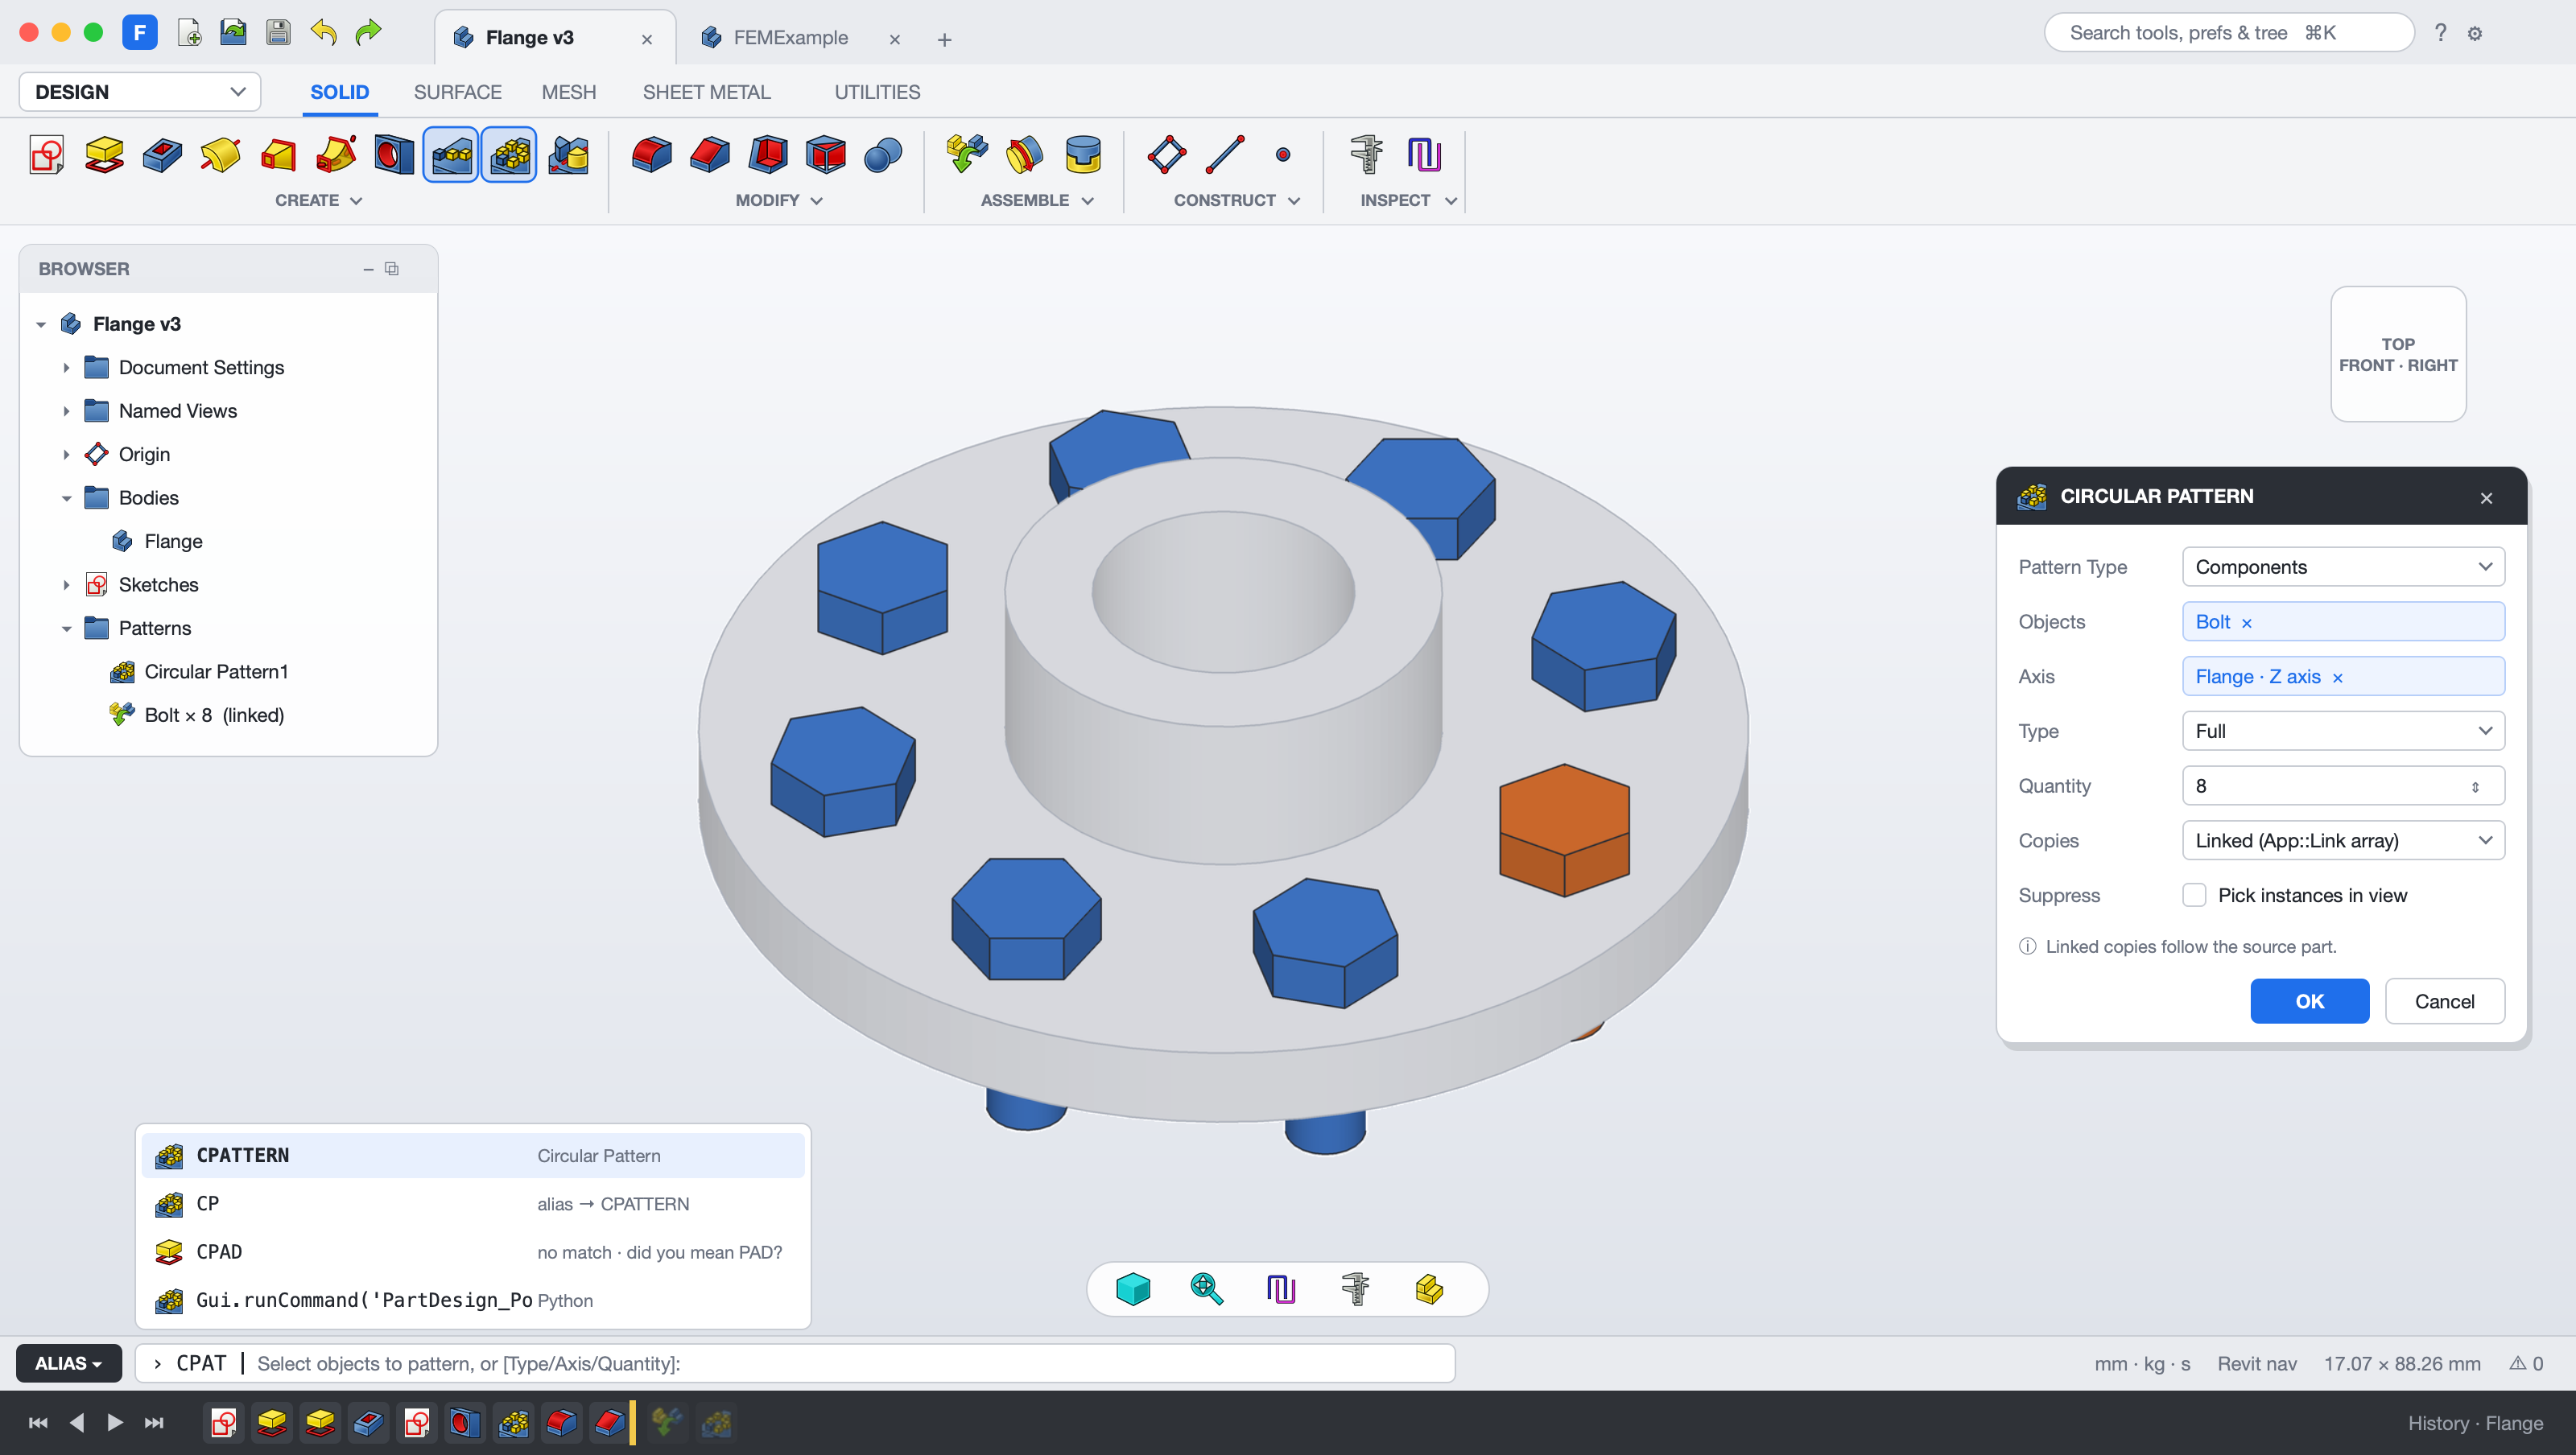
\includegraphics[width=\linewidth]{fig/layout_proposed.png}
\caption{Working mock of the Fusion-style layout: document tabs and search in the title bar; workspace
selector and tabs; captioned tool groups (Rectangular and Circular Pattern inside \textsc{Create}); Browser
top-left; floating command dialog; navigation pill; command line; timeline. FreeCAD's own icons, drawn
offscreen.}
\label{fig:after}
\end{figure}

\begin{center}
\small
\begin{tabularx}{\linewidth}{@{}llX@{}}
\toprule
Workspace & Tab & Built from\\
\midrule
\textbf{Design} & Solid & PartDesign, Part booleans, Assembly (\textsc{Assemble}), datums (\textsc{Construct}), Measure (\textsc{Inspect})\\
 & Surface & Surface workbench + Part surface tools\\
 & Mesh & Mesh and MeshPart\\
 & Sheet Metal & SheetMetal add-on (bundled)\\
 & Utilities & Spreadsheet, macros, Material, parameters (\eref{MOD-02})\\
 & \emph{Sketch} & Contextual while a sketch is open\\
\textbf{Simulation} & --- & FEM, with the study templates of \eref{SIM-01}\\
\textbf{Manufacture} & --- & CAM, print prep, flats (\S\ref{sec:mfg})\\
\textbf{Drawing} & --- & TechDraw (\S\ref{sec:drw})\\
\emph{More\ldots} & --- & Each extra workbench toggled on Preferences $\rightarrow$ BruceWorx $\rightarrow$ Workspaces\\
\bottomrule
\end{tabularx}
\end{center}

\paragraph{Selector model.} A workspace $w$ fixes a workbench $\beta(w)$, and a tab $t$ fixes a toolbar set
$\tau(w,t)$. Entering sketch edit pushes the contextual tab, and leaving pops it. Switching tabs within one
$\beta$ never switches workbench, so there is no toolbar rebuild or flicker. Implementation: a C++
\code{WorkspaceSelector} (selector type 2), a \file{workspaces.json} mapping, and a Python
\code{WorkbenchManipulator} that composes tabs from several workbenches.
